% Relatório da Atividade Prática 3 - IN1097 (Tópicos Avançados em Agentes Inteligentes 2)
% Compila com pdfLaTeX (ex.: Overleaf). As figuras ficam em figuras/ (cópias de ../results/figures/*.pdf).
% Se houver um logo do CIn no projeto (logo-cin.png), ele entra no cabeçalho; senão, o cabeçalho usa texto.
\documentclass[10pt,a4paper]{article}

\usepackage[utf8]{inputenc}
\usepackage[T1]{fontenc}
\usepackage[brazil]{babel}
\usepackage{newtxtext,newtxmath}
\usepackage{icomma}
\usepackage{amsmath}
\usepackage[a4paper,top=2.2cm,bottom=1.9cm,left=1.9cm,right=1.9cm,headheight=24pt,headsep=8pt,footskip=18pt]{geometry}
\usepackage{graphicx}
\usepackage{booktabs}
\usepackage{multirow}
\usepackage{xcolor}
\usepackage[font={small,sf},labelfont=bf,labelsep=period,skip=4pt]{caption}
\usepackage{titlesec}
\usepackage{fancyhdr}
\usepackage{microtype}
\usepackage[colorlinks=true,urlcolor=blue!60!black,linkcolor=black]{hyperref}

\graphicspath{{figuras/}}
\setlength{\parindent}{0pt}
\setlength{\parskip}{4pt}
\setlength{\textfloatsep}{8pt plus 2pt minus 2pt}
\setlength{\floatsep}{6pt plus 2pt minus 2pt}

\titleformat{\section}{\large\bfseries}{\thesection.}{0.5em}{}
\titleformat{\subsection}{\normalsize\bfseries}{\thesubsection}{0.5em}{}
\titlespacing*{\section}{0pt}{8pt}{2pt}
\titlespacing*{\subsection}{0pt}{6pt}{1pt}

\pagestyle{fancy}
\fancyhf{}
\fancyhead[L]{\IfFileExists{logo-cin.png}{\includegraphics[height=20pt]{logo-cin.png}}{\small\bfseries Centro de Informática --- UFPE}}
\fancyhead[R]{\small Tópicos Avançados em Agentes Inteligentes 2\\ ATIVIDADE PRÁTICA 3}
\fancyfoot[L]{\small 2026.2}
\fancyfoot[C]{\small IN1097}
\fancyfoot[R]{\small Johnattan D. F. Viana}
\renewcommand{\headrulewidth}{0.5pt}

\newcommand{\ninit}{n_{\text{init}}}
\newcommand{\pholm}{p_{\text{Holm}}}

\begin{document}

\begin{center}
{\Large\bfseries Warm-starting da otimização de hiperparâmetros}\\[4pt]
Johnattan D. F. Viana (\texttt{jdfv@cin.ufpe.br})\\[1pt]
{\small Código, notebooks executados e matriz de perdas:
\href{https://github.com/johnattandouglas/DisciplinaMtL/tree/main/entrega3}{github.com/johnattandouglas/DisciplinaMtL/tree/main/entrega3}}
\end{center}

%=======================================================================================================================
\section{Os meta-dados}

\textbf{Problema e datasets.} Trocamos o problema das Atividades 1 e 2 pela meta-task de \textit{warm-start} de HPO do paper do
Dataset2Vec (D2V) [Jomaa et al. 2021, \S6.3], que é a tarefa em que a pesquisa avalia representações de datasets. São 120
datasets de classificação do UCI --- a coleção pré-processada de Fernández-Delgado et al. (2014), a mesma de onde vieram os 30
datasets da Atividade~1 ---, com 16 a 130.064 instâncias (mediana 687), 3 a 262 atributos e 2 a 100 classes. A pergunta passa a
ser \textit{com qual configuração começar a busca} de um algoritmo já escolhido.

\textbf{Algoritmo e espaço $\Theta$.} O algoritmo base é uma rede \textit{feed-forward} (MLP) treinada por 50 épocas --- o
algoritmo da meta-task do D2V e um dos candidatos da Atividade~2. $\Theta$ tem 7 hiperparâmetros: ativação \{ReLU, Leaky ReLU,
SeLU\}, forma da arquitetura \{ASC, DES, ENC, SQU, SYM\}, dropout \{0; 0,2; 0,5\}, camadas \{1, 3, 5, 7\}, neurônios \{4, 8, 16,
32\}, batch-norm \{não, sim\} e otimizador \{Adam, RMSProp, SGD\}. As $\boldsymbol{K = 3456}$ configurações são o \textbf{grid
completo} (com 1 camada só existe a forma SQU, por isso não são 4320). A grade se justifica por ser o fatorial completo do
meta-dataset: a matriz fica completa, sem imputação, e $L^*$ é exato. A \textbf{configuração padrão} é o ponto do grid mais
próximo do default do \texttt{MLPClassifier} do scikit-learn (1 camada de 100 neurônios, ReLU, Adam, sem dropout/batch-norm):
ReLU, SQU, dropout 0, 1 camada de 32 neurônios (a maior largura do grid), sem batch-norm, Adam.

\textbf{Protocolo e custo.} Todas as $K \times n$ células seguem o mesmo protocolo: a configuração é treinada na partição de
treino do dataset e avaliada no hold-out de validação fixo do meta-dataset; \textbf{perda = 1 $-$ acurácia de validação na
época 50}. A matriz $K \times n = 3456 \times 120$ (\texttt{results/matriz\_de\_perdas.csv}) equivale a \textbf{414.720 treinos
de 50 épocas}, pré-computados pelos autores do meta-dataset; nosso custo foi baixar $\sim$1~GB e \textit{canonizar} o grid (cada
arquivo traz as configurações em outra ordem, e alguns repetem configurações). Usamos $\boldsymbol{T = 100}$ avaliações por busca
($K = 3456 \gg 3T = 300$) e $\boldsymbol{\ninit = 20}$ pontos iniciais (o protocolo do D2V), com \textbf{5 sementes} por
(método, alvo). A matriz tem pouca resolução no topo: a mediana é de 44 valores distintos de perda por dataset (partições de
validação pequenas) e em 18 datasets $\geq 1\%$ das configurações empatam no ótimo --- empates que desfazemos por sorteio com a
semente.

%=======================================================================================================================
\section{Métodos}

Para cada alvo $d_t$ (leave-one-dataset-out), avaliar uma configuração é ler a célula de $d_t$; todo o meta-conhecimento
(vizinhos, ranks médios, normalização das meta-características) vem só dos outros 119. Comparamos: (1)~\textbf{Padrão};
(2)~\textbf{Random Search} sem reposição; (3)~\textbf{SMBO frio}, 20 configurações aleatórias + SMBO;
(4)~\textbf{WS-$\langle$rep$\rangle$}, cujos 20 pontos iniciais vêm dos $k$ datasets mais próximos de $d_t$ no espaço
$\langle$rep$\rangle$, em rodízio (a melhor configuração de cada vizinho, depois a 2\textsuperscript{a} melhor de cada um,
\ldots; com $k = 1$ são as 20 melhores do vizinho mais próximo, como no D2V, e com $k \geq 20$ seria exatamente Feurer et al.
(2014)); e (5)~\textbf{WS independente}, as 20 configurações de melhor rank médio nos 119 datasets de treino. Os métodos 3--5 usam
o mesmo SMBO: \textbf{GP com kernel Matérn 3/2 e ARD} (hiperparâmetros reotimizados a cada iteração) sobre a codificação one-hot
das configurações e \textbf{Expected Improvement} sobre as configurações ainda não avaliadas. A comparação principal usa
$\boldsymbol{k = 1}$, fixado a priori; $k \in \{1, 3, 5\}$ entra na Análise~2, junto com um controle extra,
\textbf{WS-Random}: o método 4 com uma representação aleatória (32 dims $\sim \mathcal{U}(-1, 1)$), isto é, $k$ datasets
\textit{arbitrários} no lugar dos mais similares.

\textbf{Meta-características.} \textit{Clássicas}: \textbf{PyMFE} (\texttt{MFE()} padrão [Alcobaça et al. 2020]; 102 colunas
após a limpeza), \textbf{MF1} (Wistuba et al. 2016; 28) e \textbf{MF2} (Feurer et al. 2015; 22). \textit{Aprendidas}:
\textbf{D2V} (32 dims) e a nossa \textbf{Our-Trained} (1024 dims): um encoder de atenção invariante a permutações sobre o dataset
bruto $\rightarrow$ MLP $\rightarrow$ $z$, treinado com entropia cruzada para prever, para cada um dos 7 hiperparâmetros, a
distribuição de valores entre as 20 melhores configurações do dataset --- um alvo específico desta meta-task. D2V e Our-Trained têm
um extrator por split oficial do D2V (80/16/24 datasets de treino/validação/teste); o alvo usa o extrator do split em que ele é de
teste, que nunca o viu. Para cada alvo, descarte de colunas com NaN, imputação e min-max são ajustados nos outros 119; a distância
é euclidiana.

\textbf{Métricas.} Perda normalizada da melhor configuração até a avaliação $i$, $(L - L^*)/(L_{\text{pior}} - L^*)$ por dataset,
média sobre sementes e datasets (o ADTM do D2V); \textbf{AUC} = média dessa curva em $i = 1..T$; rank médio entre métodos (a outra
métrica do D2V). Testes: Friedman com diferença crítica de Nemenyi [Demšar 2006] ($\alpha = 0,05$; $N = 120$ datasets como
blocos, sementes agregadas pela média) e Wilcoxon pareado com correção de Holm para os pares de interesse.

%=======================================================================================================================
\section{Resultados}
\subsection{Análise 1 --- Curvas de perda}

\begin{figure}[!htb]
\centering
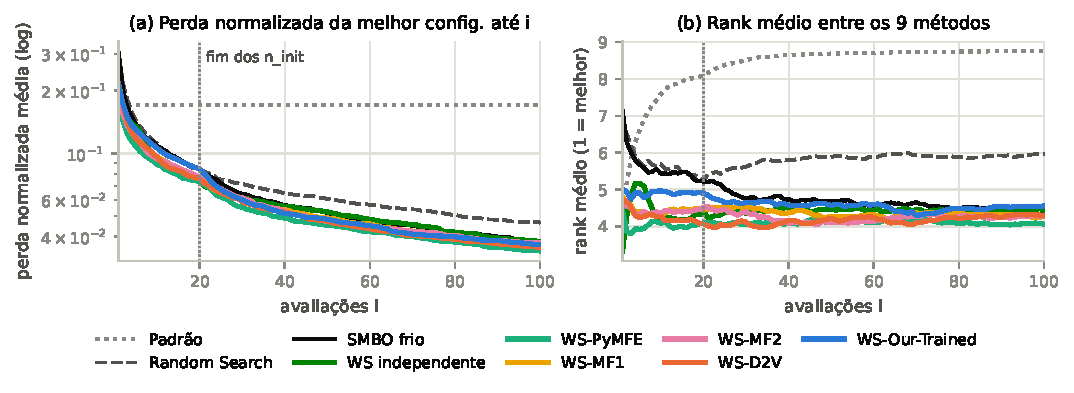
\includegraphics[width=\textwidth]{analise1_curvas.pdf}
\caption{(a) Perda normalizada da melhor configuração até a avaliação $i$ (média sobre 120 alvos $\times$ 5 sementes; escala log)
e (b) rank médio entre os 9 métodos a cada avaliação. Warm-start por similaridade com $k = 1$. A linha pontilhada vertical marca o
fim dos $\ninit = 20$ pontos iniciais.}
\label{fig:curvas}
\end{figure}

\begin{table}[!htb]
\centering
\caption{Perda normalizada média logo após os pontos iniciais ($t = 20$), em um orçamento intermediário ($t = 50$) e em
$T = 100$; AUC = média da curva em $i = 1..100$; rank médio da AUC entre os 9 métodos. Menor = melhor; \dag\ = melhor que o SMBO
frio (Wilcoxon pareado, Holm, $\alpha = 0,05$).}
\label{tab:analise1}
\small
\begin{tabular}{lrrrrr}
\toprule
Método & $t = 20$ & $t = 50$ & $t = 100$ & AUC & rank (AUC) \\
\midrule
WS-PyMFE & \textbf{0,073}\,\dag & \textbf{0,045} & \textbf{0,034} & \textbf{0,055}\,\dag & \textbf{3,95} \\
WS-D2V & 0,076\,\dag & 0,048 & 0,035 & 0,058 & 4,01 \\
WS-MF2 & 0,077 & 0,047 & 0,037 & 0,059 & 4,19 \\
WS-MF1 & 0,077 & 0,049 & 0,036 & 0,059 & 4,35 \\
WS-Our-Trained & 0,085 & 0,048 & 0,037 & 0,061 & 4,53 \\
\midrule
WS independente (método 5) & 0,076 & 0,053 & 0,038 & 0,060 & 4,14 \\
SMBO frio (método 3) & 0,084 & 0,052 & 0,038 & 0,065 & 5,40 \\
Random Search (método 2) & 0,083 & 0,061 & 0,047 & 0,072 & 6,07 \\
Padrão (método 1) & 0,170 & 0,170 & 0,170 & 0,170 & 8,36 \\
\bottomrule
\end{tabular}
\end{table}

\begin{figure}[!htb]
\centering
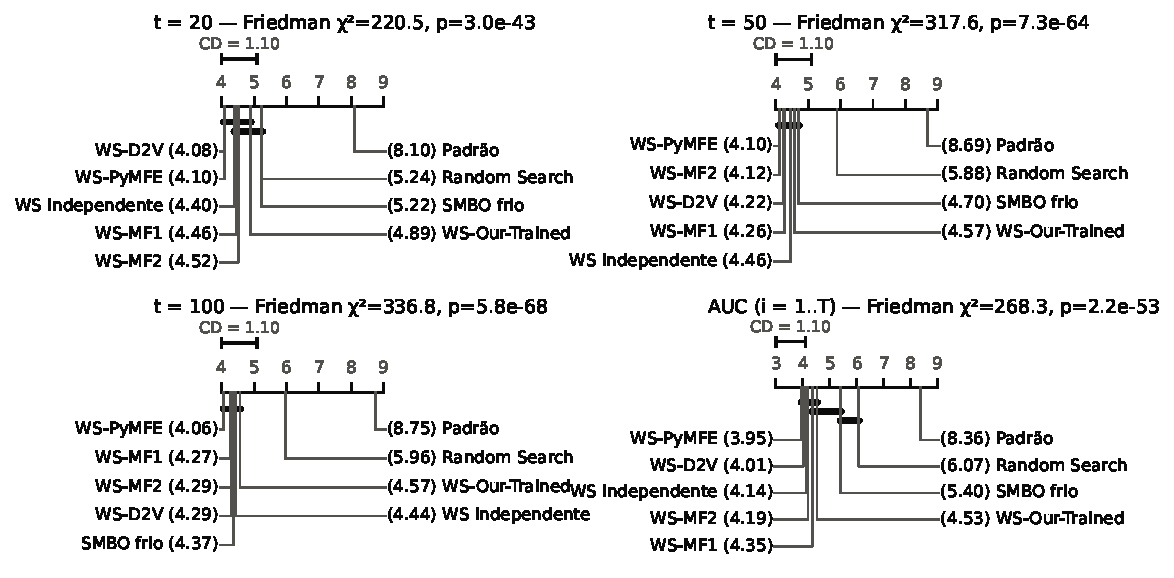
\includegraphics[width=0.88\textwidth]{analise1_cd.pdf}
\caption{Diagramas de diferença crítica (Friedman + Nemenyi, $\alpha = 0,05$, $N = 120$, CD = 1,10) em $t = 20$, $t = 50$,
$t = 100$ e na AUC. Barras grossas ligam métodos cuja diferença de rank médio não excede a CD.}
\label{fig:cd}
\end{figure}

O teste de Friedman rejeita a igualdade em todos os orçamentos ($\chi^2 = 220,5$ em $t = 20$ até $336,8$ em $t = 100$;
$p < 10^{-42}$), mas boa parte disso vem do Padrão e do Random Search. Entre os SMBO, o quadro muda com o orçamento.
\textbf{Logo após os pontos iniciais} ($t = 20$), os warm-starts por WS-D2V e WS-PyMFE ficam a mais de uma CD do SMBO frio e do
Random Search, e também vencem o SMBO frio no Wilcoxon-Holm ($p = 0,04$ e $0,03$); a perda média cai de 0,084 para 0,073--0,076.
Em $\boldsymbol{t = 50}$ nenhum par de SMBO difere após a correção de Holm, e em $\boldsymbol{T = 100}$ todos os SMBO formam um
único grupo (perdas de 0,034 a 0,038, $\pholm \geq 0,46$). Na AUC, que integra a curva, todos os warm-starts por similaridade,
exceto Our-Trained e MF1, ficam a mais de uma CD do SMBO frio, mas só o WS-PyMFE passa no Wilcoxon-Holm ($p = 0,002$). O rank
médio por avaliação (Fig.~\ref{fig:curvas}b) mostra a mesma coisa: os warm-starts lideram desde a 1\textsuperscript{a} avaliação e
o SMBO frio alcança o grupo perto de $i = 80$. \textbf{O warm-start ajuda no começo; a vantagem não persiste até $\boldsymbol{T}$}
--- o GP com EI recupera o atraso em $\sim$60 avaliações. O WS-Our-Trained é a exceção: em $t = 20$ ele não difere do SMBO frio
(0,085 $\times$ 0,084).

\subsection{Análise 2 --- O papel das meta-características}

\begin{table}[!htb]
\centering
\caption{Warm-start por similaridade (método 4) com $k$ vizinhos, comparado ao WS independente (método 5, $t = 20$: 0,076; AUC:
0,060) e ao controle WS-Random, que usa $k$ datasets \textit{arbitrários}. $^{*}$ = melhor que o WS independente (Wilcoxon-Holm
sobre 18 comparações); \ddag\ = melhor que o WS-Random com o mesmo $k$ (Wilcoxon-Holm sobre 30 comparações); $\alpha = 0,05$.}
\label{tab:analise2}
\small
\begin{tabular}{lrrrrrr}
\toprule
\multirow{2}{*}{Representação} & \multicolumn{3}{c}{perda em $t = 20$} & \multicolumn{3}{c}{AUC ($i = 1..100$)} \\
\cmidrule(lr){2-4} \cmidrule(lr){5-7}
 & $k = 1$ & $k = 3$ & $k = 5$ & $k = 1$ & $k = 3$ & $k = 5$ \\
\midrule
PyMFE (clássica) & 0,073 & 0,064 & 0,064 & 0,055 & 0,053 & 0,052\,\ddag \\
MF1 (clássica) & 0,077 & 0,067 & \textbf{0,060}$^{*}$ & 0,059 & 0,055 & \textbf{0,051}\,\ddag \\
MF2 (clássica) & 0,077 & 0,067 & 0,062\,\ddag & 0,059 & 0,055 & 0,052\,\ddag \\
D2V (aprendida) & 0,076 & 0,067 & 0,063 & 0,058 & 0,055 & 0,054 \\
Our-Trained (aprendida) & 0,085 & 0,069 & 0,063 & 0,061 & 0,057 & 0,054 \\
\midrule
Random (controle) & 0,082 & 0,072 & 0,071 & 0,062 & 0,059 & 0,059 \\
\bottomrule
\end{tabular}
\end{table}

\begin{figure}[!htb]
\centering
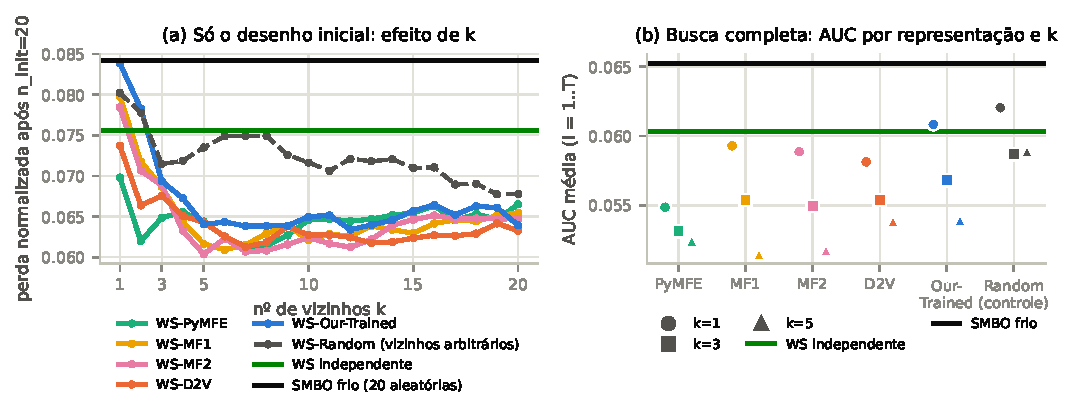
\includegraphics[width=\textwidth]{analise2_meta_caracteristicas.pdf}
\caption{(a) Só a fase inicial (sem SMBO): perda normalizada após os 20 pontos do warm-start em função do número de vizinhos $k$,
calculada exatamente para $k = 1..20$ (média sobre alvos e 5 sorteios de empates). (b) AUC da busca completa por representação e
$k$.}
\label{fig:analise2}
\end{figure}

\textbf{Método 4 $\times$ método 5.} Com $k = 1$, nenhum warm-start por similaridade difere do WS independente em orçamento algum
($\pholm \geq 0,76$ na AUC); o melhor deles, PyMFE, vence o controle em 65 alvos e perde em 54. \textbf{Clássicas $\times$
aprendidas:} a AUC média das aprendidas (0,0595) não difere da das clássicas (0,0577; Wilcoxon $p = 0,34$). O vizinho escolhido é
pouco melhor que um dataset qualquer: na matriz $M[i, j]$ (perda em $i$ usando as 20 melhores configurações de $j$), ele fica no
percentil 42 (PyMFE), 44 (D2V), 48 (MF1, MF2) e 52 (Our-Trained) dos 119 candidatos, contra 50 de um vizinho aleatório e uma perda
de 0,008 do melhor vizinho possível (oráculo) --- há muito a ganhar com um vizinho certo, e as meta-características quase não o
encontram. Só o D2V tem distância correlacionada com a utilidade do vizinho ($\rho$ médio $= 0,06$, $p = 0,0002$), e mesmo assim
fracamente --- a representação aleatória chega a $\rho = 0,02$ ($p = 0,03$); nas demais $\rho \approx 0$. As representações também
quase nunca concordam: escolhem o mesmo vizinho em 2--22\% dos alvos (MF1 e MF2, 65\%).

\textbf{Efeito de $\boldsymbol{k}$.} Aumentar $k$ ajuda todas as representações: em $t = 20$ a perda cai de 0,073--0,085
($k = 1$) para 0,060--0,064 ($k = 5$), e o WS-MF1 com $k = 5$ passa a vencer o WS independente ($\pholm = 0,01$). A
Fig.~\ref{fig:analise2}a mostra que, a partir de $k \approx 5$, as curvas de todas as representações se sobrepõem em 0,060--0,065
--- abaixo do controle com vizinhos arbitrários, que estaciona em 0,068--0,075. Há, portanto, dois efeitos. (i)~\textbf{Agregar}
as melhores configurações de vários datasets já ajuda por si: na busca completa, o WS-Random cai de 0,082 ($k = 1$) para 0,071
($k = 5$) em $t = 20$, nominalmente abaixo do WS independente. (ii)~\textbf{Escolher} esses datasets por similaridade acrescenta
um ganho que só aparece com $k = 5$: as três clássicas vencem o WS-Random na AUC (PyMFE, MF1 e MF2: $\pholm = 0,013$, $0,015$ e
$0,004$; melhores em 74--77 dos 120 alvos) e o MF2 também em $t = 20$ ($\pholm = 0,02$); D2V (0,16) e Our-Trained (0,54) não. Com
$k = 1$ ou 3, nenhuma representação supera vizinhos arbitrários ($\pholm \geq 0,49$). \textbf{A similaridade orienta a escolha,
mas fracamente:} um único vizinho é ruidoso demais, e o sinal só aparece ao agregar alguns vizinhos --- e só com as
meta-características clássicas.

\subsection{Análise 3 --- Quando o warm-start falha}

\begin{figure}[!htb]
\centering
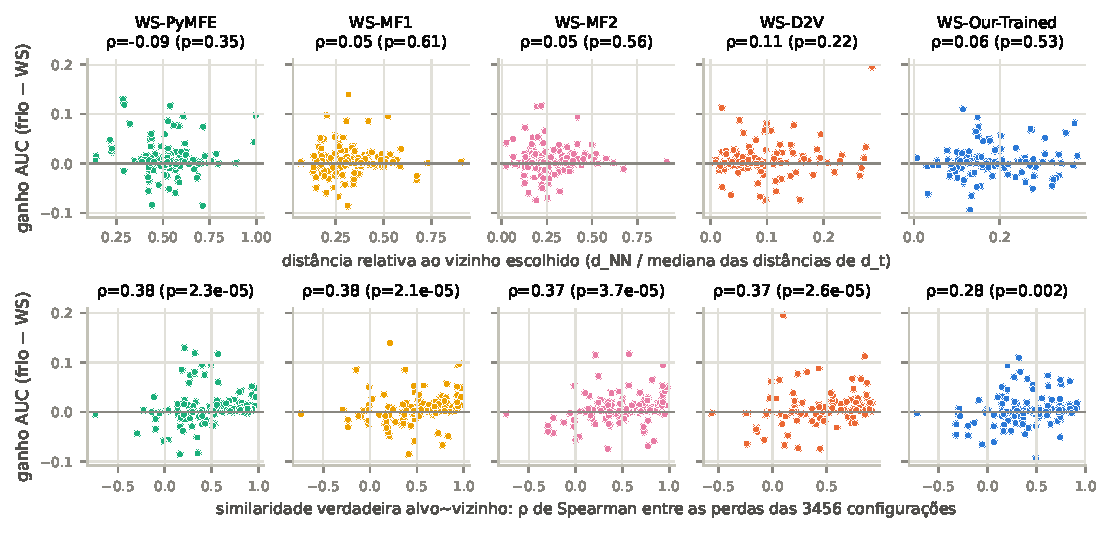
\includegraphics[width=\textwidth]{analise3_ganho_vs_distancia.pdf}
\caption{Ganho do método 4 ($k = 1$) sobre o método 3 por alvo, ganho = AUC(SMBO frio) $-$ AUC(WS) ($> 0$: o warm-start ajudou),
contra (linha de cima) a distância relativa do alvo ao vizinho escolhido e (linha de baixo) a similaridade ``verdadeira'' entre os
dois --- o $\rho$ de Spearman entre as perdas das 3456 configurações nos dois datasets.}
\label{fig:analise3}
\end{figure}

O warm-start ($k = 1$) é melhor que partir do zero em 76--82 dos 120 alvos e pior em 38--44, conforme a representação.
\textbf{O ganho não se relaciona com a distância ao vizinho} em nenhuma representação: $\rho$ de Spearman entre ganho e distância
relativa de $-0,09$ (PyMFE) a $0,11$ (D2V), todos com $p \geq 0,22$ (o mesmo com a distância absoluta). Estar ``perto'' no espaço
de meta-características não indica que o vizinho é útil. O que explica o ganho é a \textbf{similaridade verdadeira} entre as
paisagens de perda do alvo e do vizinho ($\rho = 0,28$--$0,38$ com o ganho, Fig.~\ref{fig:analise3} embaixo): nos alvos em que o
warm-start perdeu, a mediana dessa similaridade é 0,22--0,35, contra 0,60--0,72 nos alvos em que ganhou (Mann-Whitney,
$p \leq 6 \times 10^{-5}$), e os 20 pontos herdados deixam o alvo com perda 0,10--0,12, contra 0,02--0,03. Exemplos: o
Our-Trained manda \textit{cardiotocography-3clases} para \textit{bank} ($\rho = -0,32$, quando havia um vizinho com
$\rho = 0,92$) e \textit{wine-quality-white} para \textit{post-operative} ($\rho = -0,05$; melhor possível 0,81); o D2V manda
\textit{breast-cancer-wisc-prog} para \textit{oocytes\_merluccius\_nucleus\_4d} ($\rho = -0,24$). A falha depende mais do alvo do
que da representação: os ganhos das cinco representações se correlacionam ($\rho = 0,27$--$0,67$), e em 10 alvos todas perdem
para o SMBO frio --- \textit{lung-cancer}, \textit{post-operative}, \textit{heart-switzerland}, \textit{echocardiogram},
\textit{parkinsons}, \textit{contrac}, \textit{monks-1}, \textit{mammographic}, \textit{pittsburg-bridges-MATERIAL} e
\textit{vertebral-column-2clases}. São, em geral, datasets pequenos (32 a 1.473 instâncias; os alvos em que o warm-start falha
são menores que aqueles em que ele ganha, $p \leq 0,004$ para D2V e MF1): com poucas instâncias de validação a perda é ruidosa e
de baixa resolução, a paisagem de um dataset pouco diz sobre a de outro e, quando muitas configurações empatam no ótimo (9\% em
\textit{lung-cancer}), 20 pontos aleatórios já bastam.

%=======================================================================================================================
\section{Interpretação}

\textbf{O warm-start acelerou a busca?} Sim, mas só no começo. Os 20 pontos herdados reduzem a perda em $t = 20$ em até 13\% em
relação ao SMBO frio (significativo para PyMFE e D2V) e a vantagem diminui depois: em $t = 50$ já não é significativa e em
$T = 100$ todos os SMBO empatam. Ele ajuda em cerca de 2/3 dos alvos --- naqueles cuja paisagem de perda se parece com a de algum
dataset de treino --- e atrapalha nos datasets pequenos e ruidosos, em que o vizinho transfere configurações que só eram boas
para ele.

\textbf{O ganho vem das meta-características ou do portfólio?} Principalmente do portfólio. No protocolo do D2V ($k = 1$), o
warm-start por similaridade não supera nem o WS independente nem vizinhos arbitrários: o ganho sobre a partida fria vem de começar
por configurações que são boas em \textit{algum} dataset, não de achar o dataset certo --- o vizinho escolhido fica perto do
percentil 50 dos candidatos, enquanto o oráculo mostra que o vizinho certo levaria a perda inicial de 0,08 a 0,008. O sinal das
meta-características existe, mas é pequeno e só aparece com $k = 5$ e com as clássicas: perto do efeito de agregar
(0,082 $\rightarrow$ 0,071 com vizinhos arbitrários), escolhê-los por similaridade acrescenta 0,071 $\rightarrow$ 0,060--0,064 em
$t = 20$. As aprendidas não superaram as clássicas ($p = 0,34$). O próprio controle do método 5 é um portfólio fraco: o rank
médio escolhe configurações boas ``na média'' e parecidas entre si, e fica, nominalmente, atrás das melhores configurações de 5
datasets arbitrários; um portfólio guloso, que minimiza a perda do melhor ponto do conjunto, seria um controle mais exigente.

\textbf{O que a restrição às $\boldsymbol{K}$ configurações pode ter escondido.} A busca simulada torna o experimento possível ---
13.200 buscas (22 variantes $\times$ 120 alvos $\times$ 5 sementes) custaram 26,7~h de CPU (2,5~h em 11 núcleos), contra o
equivalente a $\sim$1,3 milhão de treinos reais ---, mas tem preço. (i)~$L^*$ é o ótimo \textit{do grid}: taxa de aprendizado,
tamanho do lote e número de épocas estão fixos, então não sabemos quanto o grid deixa de fora nem se o warm-start ajudaria num
espaço contínuo, onde as configurações de um vizinho não existem exatamente no alvo e teriam de ser mapeadas. (ii)~Transferir
configurações idênticas é o caso mais favorável ao warm-start; com GP sobre um espaço contínuo, o desenho inicial pesaria menos.
(iii)~O custo é contado em avaliações, não em tempo: uma rede de 7 camadas custa mais que uma de 1, e o warm-start pode herdar
configurações caras. (iv)~A resposta é de baixa resolução (mediana de 44 valores distintos de perda por dataset) e o ótimo de
validação nem sempre é o de teste: escolhê-lo custa, em mediana, 4,3~p.p. de acurácia de teste em relação ao ótimo de teste
($\rho$ validação$\sim$teste $= 0,72$) --- parte das ``melhores configurações'' transferidas é ruído de um hold-out pequeno.

\textbf{O que levo para a pesquisa.} (1)~A Our-Trained de 1024 dimensões foi o pior warm-start, e o diagnóstico de treino explica
por quê: o alvo (a distribuição dos hiperparâmetros das top-20 configurações) é previsto tão bem por uma distribuição constante
quanto pelo modelo (CE de validação 1,081--1,140 contra 1,092--1,141 do prior constante), logo nada obriga $z$ a separar datasets
--- a dimensão maior não compensa um objetivo que não exige similaridade. O objetivo deveria ser relacional, alinhando distâncias
em $z$ à similaridade de paisagem (o $\rho$ que explicou as falhas) ou à matriz de transferência $M$. (2)~Avaliar uma
representação para warm-start exige os controles de portfólio e de vizinhos arbitrários; compará-la só com a partida fria atribui
à representação um ganho que é do portfólio. (3)~Desenhos com vários vizinhos ($k = 5$) são mais robustos que copiar as 20
melhores de um só dataset, como no protocolo original do D2V --- e é só com eles que a similaridade se mostra útil.

%=======================================================================================================================
\section*{Referências}
{\small
\setlength{\parskip}{1pt}
\setlength{\leftskip}{12pt}
\setlength{\parindent}{-12pt}

Alcobaça, E. et al. (2020). MFE: towards reproducible meta-feature extraction. \textit{JMLR}, 21(111):1--5.

Demšar, J. (2006). Statistical comparisons of classifiers over multiple data sets. \textit{JMLR}, 7:1--30.

Fernández-Delgado, M., Cernadas, E., Barro, S. e Amorim, D. (2014). Do we need hundreds of classifiers to solve real world
classification problems? \textit{JMLR}, 15:3133--3181.

Feurer, M., Springenberg, J. T. e Hutter, F. (2014). Using meta-learning to initialize Bayesian optimization of hyperparameters.
\textit{MetaSel@ECAI}, 3--10.

Feurer, M., Springenberg, J. T. e Hutter, F. (2015). Initializing Bayesian hyperparameter optimization via meta-learning.
\textit{AAAI}, 1128--1135.

Jomaa, H. S., Schmidt-Thieme, L. e Grabocka, J. (2021). Dataset2Vec: learning dataset meta-features. \textit{Data Mining and
Knowledge Discovery}, 35:964--985.

Wistuba, M., Schilling, N. e Schmidt-Thieme, L. (2016). Two-stage transfer surrogate model for automatic hyperparameter
optimization. \textit{ECML-PKDD}, 199--214.
\par}

\end{document}
